\section{Exercises}
\label{section:comboBbExercises}
\graphicspath{ {./chapter04/FigHw} }

\begin{enumerate}
    \item \textbf{ (2 pts. each)}Short answer:
        \begin{enumerate}
            \item How many 3:8 decoders would it take to build a 9:512 decoder?

                \begin{onlysolution} \textbf{Solutions} \itshape{A total of 73 decoders are required.  There
                        are 512/8 = 64 on
                    the output layer, 64/8 = 8 in the middle layer and 1 on the input.}
                \end{onlysolution}
            \item How many AND gates are there in a $2^N$:1 mux?

                \begin{onlysolution} \textbf{Solutions} \itshape{ Each input requires 1 AND gate, hence $2^N$
                    AND gates.}
                \end{onlysolution}
            \item How many AND gates are there in a $2^N:1$ mux which is
                constructed out of 2:1 muxes?

                \begin{onlysolution} \textbf{Solutions} \itshape{ A $2^N$ Mux requires the following number
                        of 2:1 muxes:
                        $$ 2^N/2 + 2^N/4 + ... + 2^N/2^N = $$
                        $$ 2^N(1/2 + 1/4 + ... + 1/2^N) = $$
                        $$ 2^N(1-1/2^(N+1)) =  $$
                        $$ 2^N - 1  $$
                        Since each 2:1 mux contains 2 AND gates, the total number of AND gates is
                        $2^(N+1) - 2$.
                    }
                \end{onlysolution}

            \item How many AND gates are there in a $2^N$:1 mux which is
                constructed out of $2^L$:1 muxes, assume that
                $2^N$ is an integer multiple of $2^L$?

                \begin{onlysolution} \textbf{Solutions} \itshape{
                        A $2^N$ Mux requires the following number of $2^L:1$ muxes:
                        $$ 2^N/2^L + 2^N/2^(2L) + ... 2^N/2^(kL) $$
                        $$ 2^N(1/2^L + 1/2^(2L) + ... 1/2^(kL)) $$
                        Where $k = N/L$.  Each $2^L:1$ mux requires $2^L$ AND gates for its construction,
                        so the number of AND gates is the product of the number of $2^L:1$ muxes and the
                        number of AND gates in a single $2^L:1$ mux, or:
                        $$ 2^N * 2^L(1/2^L + 1/2^(2L) + ... 1/2^(kL)) $$
                        $$ 2^N (1 + 1/2 + ... 1/2^k) $$
                        $$ 2^N (2-1/2^(k+1)) $$
                        $$ 2^N (2-1/2^(N/L+1) $$
                            $$ 2^(N+1) - 2^(N-N/L-1) $$
                        }
                    \end{onlysolution}

            \end{enumerate}

        \item \textbf{ (6 pts.)}Determine the \SOPmin expression for each of the
            three outputs of a bit-slice of the comparator.

            \begin{onlysolution} \textbf{Solutions} \itshape{
                    The following five variable Kmap describes $E_{out}$

                    \begin{tabular}{cc}
                        $
                        \begin{array} {c||c|c|c|c}
                            L_{in} G_{in}  \bs x  y & 00 & 01 & 11 & 10 \\ \hline \hline
                            00       & x  & x  & x  &  x \\ \hline
                            01       & 0  & 0  & 0  &  0 \\ \hline
                            11       & x  & x  & x  &  x \\ \hline
                            10       & 0  & 0  & 0  &  0 \\
                        \end{array}$
                        &
                        $
                        \begin{array} {c||c|c|c|c}
                            L_{in} G_{in}  \bs x  y & 00 & 01 & 11 & 10 \\ \hline \hline
                            00       & 1  & 0  & 1  & 0  \\ \hline
                            01       & x  & x  & x  & x  \\ \hline
                            11       & x  & x  & x  & x  \\ \hline
                            10       & x  & x  & x  & x  \\
                        \end{array}$  \\
                        $E_{in}=0$ & $E_{in}=1$ \\
                        \multicolumn{2}{c}{$E_{out} = L_{in}'G_{in}'x'y' + L_{in}'G_{in}'xy $} \\
                    \end{tabular}

                    The following five variable Kmap describes $G_{out}$

                    \begin{tabular}{cc}
                        $
                        \begin{array} {c||c|c|c|c}
                            L_{in} G_{in}  \bs x  y & 00 & 01 & 11 & 10 \\ \hline \hline
                            00       & x  & x  & x  & x  \\ \hline
                            01       & 1  & 1  & 1  & 1  \\ \hline
                            11       & x  & x  & x  & x  \\ \hline
                            10       & 0  & 0  & 0  & 0  \\
                        \end{array}$
                        &
                        $
                        \begin{array} {c||c|c|c|c}
                            L_{in} G_{in}  \bs x  y & 00 & 01 & 11 & 10 \\ \hline \hline
                            00       & 0  & 0  & 0  & 1  \\ \hline
                            01       & x  & x  & x  & x  \\ \hline
                            11       & x  & x  & x  & x  \\ \hline
                            10       & x  & x  & x  & x  \\
                        \end{array}$  \\
                        $E_{in}=0$ & $E_{in}=1$ \\
                        \multicolumn{2}{c}{$G_{out} = G_{in} + L_{in}'xy'$} \\
                    \end{tabular}

                    The following five variable Kmap describes $L_{out}$

                    \begin{tabular}{cc}
                        $
                        \begin{array} {c||c|c|c|c}
                            L_{in} G_{in}  \bs x  y & 00 & 01 & 11 & 10 \\ \hline \hline
                            00       & x  & x  & x  & x  \\ \hline
                            01       & 0  & 0  & 0  & 0  \\ \hline
                            11       & x  & x  & x  & x  \\ \hline
                            10       & 1  & 1  & 1  & 1  \\
                        \end{array}$
                        &
                        $
                        \begin{array} {c||c|c|c|c}
                            L_{in} G_{in}  \bs x  y & 00 & 01 & 11 & 10 \\ \hline \hline
                            00       & 0  & 1  & 0  & 0  \\ \hline
                            01       & x  & x  & x  & x  \\ \hline
                            11       & x  & x  & x  & x  \\ \hline
                            10       & x  & x  & x  & x  \\
                        \end{array}$  \\
                        $E_{in}=0$ & $E_{in}=1$ \\
                        \multicolumn{2}{c}{$L_{out} = L_{in} + G_{in}'x'y$} \\
                    \end{tabular}
                }
            \end{onlysolution}

        \item \textbf{ (2 pts.)}Show how to connect together four 4-bit comparators to
            construct a 16-bit comparator.

            \begin{onlysolution} \textbf{Solutions} \itshape{ Figure forthcoming}
            \end{onlysolution}

        \item \textbf{ (2 pts.)}Determine the circuitry for the overflow detection
            circuit for a 2's-complement adder subtractor.  See page~\pageref{page:Ovf}.

            \begin{onlysolution} \textbf{Solutions} \itshape{
                    $
                    \begin{array} {c||c|c} \\
                        c_{in}  \bs c_{out} & 0 & 1 \\ \hline
                        0    &   & 1 \\ \hline
                        1    & 1 &   \\
                    \end{array}$   \\
                    Thus $ovf = c_{in}' c_{out} + c_{in} c_{out}' =  c_{in} \oplus c_{out} $
                }
            \end{onlysolution}

        \item \textbf{ (10 pts.)}Build a BCD to 7-Segment Display converter using
            Espresso.

            \begin{buildingblock}{BCD to 7-segment}
                \index{bcd to 7-segment}
                \label{page:7seg}
                \begin{tabular}{|l|p{3.5in}|} \hline
                    Nomenclature:  & BCD to 7-segment converter                \\ \hline
                    Data Input:    & 4-bit vector $D=d_3 d_2 d_1 d_0$  \\ \hline
                    Data Output:   & 7-bit vector $Y=y_6 \ldots y_1 y_0$    \\ \hline
                    Control:       & none                                   \\ \hline
                    Status:        & none                                   \\ \hline
                    Behavior:      & The output drives a 7-segment display pattern
                    representing the BCD digit.  \\ \hline
                \end{tabular}
            \end{buildingblock}

            A binary coded digit (BCD) is a 4-bit binary number that is constrained
            to assume the values of 0-9. That is, 1010 ... 1111 are illegal BCD digits.

            A 7-segment display is a box with seven inputs and seven output LED bars.
            Each input is wired to an LED bar that is illuminated when a 1 is applied
            to its input.
            Each of the seven LED segments is numbered according to the pattern shown
            on the left-hand side of Figure~\ref{fig:BCD}.

            \begin{figure}[ht]
                \center{\scalebox{0.7}{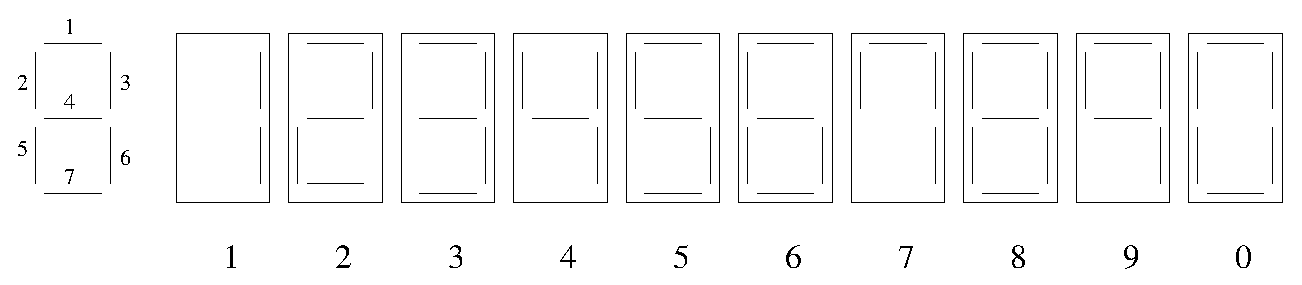
\includegraphics{Prob4-5}}}
                \caption{The numbering of the segments in a 7-segment display.
                The patterns of the BCD digits.}
                \label{fig:BCD}
            \end{figure}

            The pattern of LEDs to illuminate for each BCD digit is shown on the
            right-hand side of Figure~\ref{fig:BCD}.  A BCD to 7-segment converter
            has four inputs, $d_3 d_2 d_1 d_0$ and seven outputs $S_7 \ldots S_1$.
            Complete the design using Espresso.  Make sure to include ``Don't cares"
            in the truth table specification.
            \begin{enumerate}
                \item Use Espresso to determine the \SOPmin expression for the outputs
                    $S_7 \ldots S_1$.  Underline product terms that are shared.
                    Submit the Espresso source file.

                    \begin{onlysolution} \textbf{Solutions} \itshape{
                            The following is the source file for the BCD to 7-segment converter.

%% \begin{verbatim}
%% # BCD to 7-segment display
%% #
%% .i 4
%% .o 7
%% .ilb b3 b2 b1 b0
%% .ob  s7 s6 s5 s4 s3 s2 s1
%% 0000 1110111
%% 0001 0100100
%% 0010 1011101
%% 0011 1101101
%% 0100 0101110
%% 0101 1101011
%% 0110 1111011
%% 0111 0100111
%% 1000 1111111
%% 1001 0101111
%% 101- -------
%% 11-- -------
%% .e
%% \end{verbatim}

                            The following is the output from espresso on the
                            BCD to 7-segment converter.

%% \begin{verbatim}
%% .i 4
%% .o 7
%% .ilb b3 b2 b1 b0
%% .ob s7 s6 s5 s4 s3 s2 s1
%% .p 9
%% --11 0100100
%% -00- 0100100
%% -000 1010011
%% --10 1011000
%% -100 0101110
%% -11- 0100011
%% -101 1101011
%% -01- 1001101
%% 1--- 0001011
%% .e
%% \end{verbatim}
                        }
                    \end{onlysolution}

                \item Use Espresso to determine the \POSmin expression for the outputs
                    $S_7 \ldots S_1$.  Underline sum terms that are shared.
                    Submit the Espresso source file
                    \begin{onlysolution} \textbf{Solutions} \itshape {
                            The following output was generated by using the same file
                            as the solution in the previous part; but using the epos
                            option in espresso.

%% \begin{verbatim}
%% # BCD to 7-segment display
%% #
%% .i 4
%% .o 7
%% .ilb b3 b2 b1 b0
%% .ob s7 s6 s5 s4 s3 s2 s1
%% #.phase 0000000
%% .p 9
%% 000- 0001000
%% -110 0000100
%% -010 0100010
%% -101 0010100
%% 0001 1010011
%% -011 0010010
%% -100 1010001
%% 1--1 1010000
%% -111 1011000
%% .e
%% \end{verbatim}

                            Remember that these are the negation of the output variables, hence
                            we have to use DeMorgan's to put them into \POSmin form.
                            Symbolically we have:
%% \begin{verbatim}
s7=(b3+b2+b1+b0')(b2'+b1+b0)(b3'+b0')(b2'+b1'+b0'); \\
s6=(b2+b1'+b0); \\
s5=(b2'+b1+b0')(b3+b2+b1+b0')(b2+b1+b0')(b2'+b1+b0)(b3'+b0')(b2'+b1'+b0'); \\
s4=(b3+b2+b1)(b2'+b1'+b0'); \\
s3=(b2'+b1'+b0)(b2'+b1+b0'); \\
s2=(b2+b1'+b0)(b3+b2+b1+b0')(b2+b1'+b0'); \\
s1=(b3+b2+b1+b0')(b2'+b1+b0); \\
%% \end{verbatim}
                        }
                    \end{onlysolution}
            \end{enumerate}

        \item \textbf{ (10 pts.)} Build a box which has one 4-bit input called A and
            one 4-bit output called T. The output T is the 2's-complement value
            of the input A.  Use the bit slice paradigm to solve this
            problem.  That is, create a building block for one bit of the problem
            then string four of them together to solve the problem.
            For the problem at hand this can be done as follows:
            \begin{enumerate}
                \item Start at the LSB of A.
                \item If this is the first, least significant, 1, flip all bits
                    to the left.
                \item If this is not the first 1, leave the bit alone.
                \item Move one bit to the left.
                \item Goto Step b.
            \end{enumerate}
            A bit-slice should communicate whether there has been a 1 to the right,
            to the more significant bit.  Submit:
            \begin{itemize}
                \item How the above "algorithm" behaves when presented with
                    the inputs A=1100
                \item The truth table for one bit slice
                \item \SOPmin expression and circuit diagram for a bit slice.
                \item The organization of four bit slices to solve the problem
            \end{itemize}

            \begin{onlysolution} \textbf{Solutions} \itshape{
                    The key to the begin solution  is to figure out the structure
                    of the begin solution  and then give meaning to the signals involved.
                    The problem will be sliced into four bit-slices; each handled
                    but its own complement box.  Thus, there will be four complement
                    box in the begin solution.  Each box will have 2 inputs, one being
                    a bit of A and the other being a "carry in" from the less
                    significant less, immediately to the right.  Each box
                    will have two bits of output, a bit of T and a "carry out".
                    The carry bits (both into and out of a box will convey
                        information regarding the rightmost 1 in the number A.

                        If the carry in is equal 1 then there is a one to the right.
                        If the carry in is equal 0 then there is not a one to the right.
                        The truth table for a box is then

                        \begin{table}
                            \begin{tabular}{l|l||l|l|l}
                                $A$ & $c_{in}$  & $T$ & $c_{out}$ & comment \\ \hline
                                0   & 0       &   0 & 0          & There is no 1 to the right \\ \hline
                                0   & 1       &   1 & 1          & There is a 1 to the right, flip A \\ \hline
                                1   & 0       &   1 & 1          & There is is no 1 to the right, but we've
                                created one \\ \hline
                                1   & 1       &   0 & 1          & There is a 1 to the right, flip A \\
                            \end{tabular}
                        \end{table}

                        From this it follows that: \\
                        $T=A'c_{in} + A c_{in}'=A \oplus c_{in}$ \\
                        $c_{out} = A + c_{in}$
                    }
                \end{onlysolution}

            \item \textbf{ (4 pts.)} Build a 7:128 decoder using a minimum number of
                4:16, 2:4 and 1:2 decoders. Describe the wiring of the select lines.
                \begin{onlysolution} \textbf{Solutions} \itshape {

                        \begin{figure}[ht]
                            \center{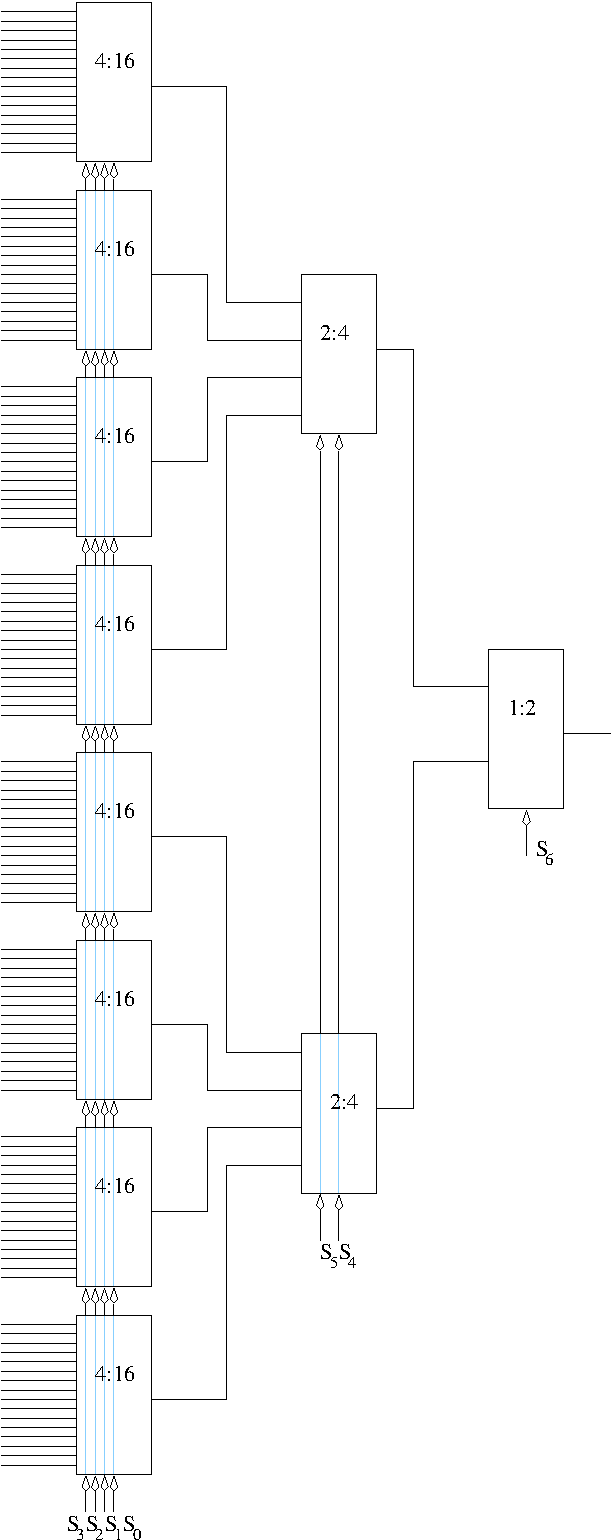
\includegraphics{Sol4-7}}
                            \caption{A 7:128 decoder built from 4:16, 2:4 and 1:2 decoders.}
                            \label{fig:bighwdec}
                        \end{figure}
                    }
                \end{onlysolution}

            \item \textbf{ (4 pts. each)} Design a circuit with two 8-bit inputs $X,Y$, an
                8-bit output $Z$ and a 1-bit input $sel$.  Construct a circuit that yields the
                correct value of $Z$ using only the basic building blocks presented in this
                chapter; do NOT show the internal organization of these building blocks.  If
                a mux is used, denote which input is the $y_0$ and which is $y_1$.
                If a comparator is used denote which input is $X$ and which is $Y$.
                Do not use any AND or OR gates; it will tempting in the later problems.
                \begin{enumerate}
                    \item \verb^ if (sel==0) then Z = X else Z = Y ^

                        \begin{onlysolution} \textbf{Solutions} \itshape{
                                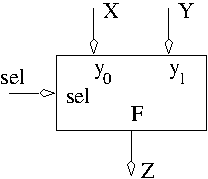
\includegraphics{Sol4-8a}
                            }
                        \end{onlysolution}

                    \item \verb^ if (sel==0) then Z = X+Y else Z = Y ^

                        \begin{onlysolution} \textbf{Solutions} \itshape{
                                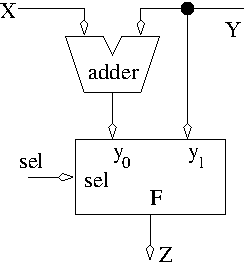
\includegraphics{Sol4-8b}
                            }
                        \end{onlysolution}

                    \item \verb^ if (sel==0) then Z = X+Y else Z = X-Y ^

                        \begin{onlysolution} \textbf{Solutions} \itshape{
                                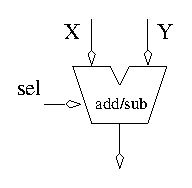
\includegraphics{Sol4-8c}
                            }
                        \end{onlysolution}

                    \item \verb^ if (X==0) then Z = X else Z = Y ^

                        \begin{onlysolution} \textbf{Solutions} \itshape{
                                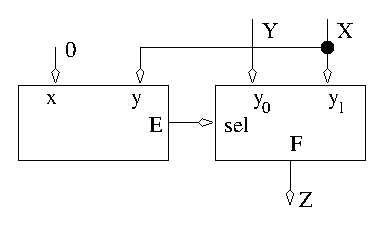
\includegraphics{Sol4-8d}
                            }
                        \end{onlysolution}

                    \item \verb^ if (X==Y) then Z = X-Y else Z = Y ^

                        \begin{onlysolution} \textbf{Solutions} \itshape{
                                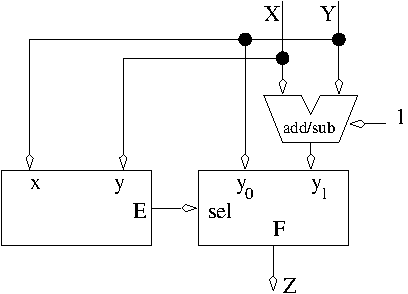
\includegraphics{Sol4-8e}
                            }
                        \end{onlysolution}

                    \item \verb^ if (X==Y) then Z = X+Y else Z = X-Y ^

                        \begin{onlysolution} \textbf{Solutions} \itshape{
                                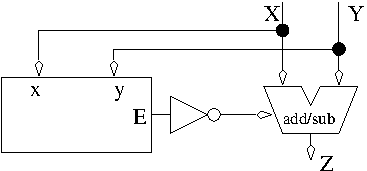
\includegraphics{Sol4-8f}
                            }
                        \end{onlysolution}

                    \item \verb^ if (X < Y) then Z = X else Z = Y ^

                        \begin{onlysolution} \textbf{Solutions} \itshape{
                                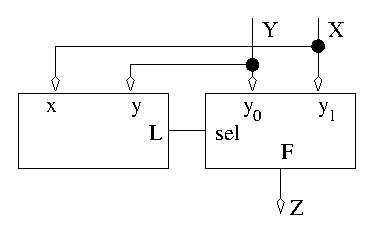
\includegraphics{Sol4-8g}
                            }
                        \end{onlysolution}

                    \item \verb^ if (X <= Y) then Z = X else Z = Y ^

                        \begin{onlysolution} \textbf{Solutions} \itshape{
                                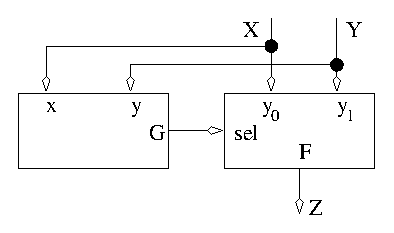
\includegraphics{Sol4-8h}
                            }
                        \end{onlysolution}

                    \item \verb^ if (X > Y) then Z = X else Z = Y ^

                        \begin{onlysolution} \textbf{Solutions} \itshape{
                                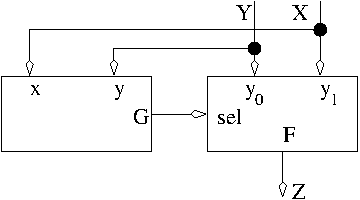
\includegraphics{Sol4-8i}
                            }
                        \end{onlysolution}

                    \item \verb^ if (X > Y) then Z = X+X else Z = Y+Y ^

                        \begin{onlysolution} \textbf{Solutions} \itshape{
                                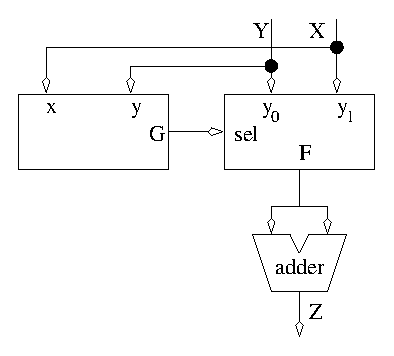
\includegraphics{Sol4-8j}
                            }
                        \end{onlysolution}

                \end{enumerate}

            \item \textbf{ (10 pts.)} Build a 4-bit priority encoder.

                \begin{buildingblock}{Priority Encoder}
                    \index{priority encoder}
                    \begin{tabular}{|l|p{3.5in}|} \hline
                        Nomenclature:  & N-bit priority encoder                \\ \hline
                        Data Input:    & N-bit vectored  $D=d_{N-1} \ldots d_1 d_0$  \\ \hline
                        Data Output:   & $\log_2(N)$-bit vector $Y=y_{log_2(N)} \ldots y_1 y_0$    \\ \hline
                        Control:       & none                    \\ \hline
                        Status:        & none                                   \\ \hline
                        Behavior:      & $F = i$ where $i$ is the highest indexed input
                        which equals 1.  When all inputs equal
                        0, the output is a ``don't care".  \\ \hline
                    \end{tabular}
                    \label{page:prior}
                \end{buildingblock}

                The idea is for the outputs to represent (in binary code) the highest
                input index which equals 1.  For example, a 4-bit priority encoder
                with input $D=1010$ has inputs $d_3=1$ and $d_0=1$.  Of these two
                inputs, the index of $d_3$ is greater than the index of $d_0$ so the
                output, $F$ is equal to 3, or in binary $11$.  If the input were
                $D=0111$ then $F=10$.

                \begin{enumerate}
                    \item Write down the truth table for a 4-bit priority encoder.  Hint,
                        the truth table could be structured so that it contains only five rows
                        by using ``don't cares" on the inputs.

                        \begin{onlysolution} \textbf{Solutions} \itshape{
                                \begin{tabular}{l|l|l|l||l|l}
                                    $d_3$ & $d_2$ & $d_1$ & $d_0$ & $f_1$ & $F_0$ \\ \hline
                                    0  &    0  &    0  &    0  &    x  &    x  \\ \hline
                                    0  &    0  &    0  &    1  &    0  &    0  \\ \hline
                                    0  &    0  &    1  &    x  &    0  &    1  \\ \hline
                                    0  &    1  &    x  &    x  &    1  &    0  \\ \hline
                                    1  &    x  &    x  &    x  &    1  &    1  \\
                                \end{tabular}
                            }
                        \end{onlysolution}

                    \item An \SOPmin realization of the circuit.
                        \begin{onlysolution} \textbf{Solutions} \itshape{
                                $f_1 = d_3 + d_2$ \\
                                $f_0 = d_3 + d_2'd_1$
                            }
                        \end{onlysolution}
                \end{enumerate}

            \item \textbf{ (10 pts.)} Build a 4-bit saturation adder.  A
                saturation adder performs normal 4-bit addition when the
                resulting sum is less than 15.  If the sum is
                greater than 15, the saturation adders outputs 15.  The
                following table summarizes.

                \begin{buildingblock}{Saturation Adder}
                    \index{saturation adder}
                    \label{page:saturation}
                    \begin{tabular}{|l|p{3.5in}|} \hline
                        Nomenclature:  & 4-bit saturation adder                \\ \hline
                        Data Input:    & 2, 4-bit vectors \verb+A, B+  \\ \hline
                        Data Output:   & 4-bit vector \verb+sum+    \\ \hline
                        Control:       & none                                   \\ \hline
                        Status:        & none                                   \\ \hline
                        Behavior:      &
                \begin{verbatim}
                if (A+B > 15) sum = 15
                else sum = A+B
                \end{verbatim}
                        \\ \hline
                    \end{tabular}
                \end{buildingblock}

                Submit a schematic showing the basic building blocks, their
                data status, and control interconnections.  Show any truth
                tables used to build glue logic.

                \begin{onlysolution} \textbf{Solutions} \itshape{
                        All we need to do is to determine when the sum is greater then
                        15 and output 15 when it is.  The comparator/mux combo mentioned
                        several times in the chapter should do the trick.

                        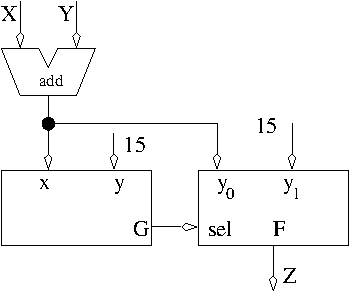
\includegraphics{Sol4-10}

                    }
                \end{onlysolution}

            \item \textbf{ (10 pts.)} Build a mod-6 adder.  The mod-6 adder
                takes as input two 3-bit (mod 6) numbers and adds them together
                modulus 6.

                \index{modular arithmetic}
                \label{page:mod}
                Modular arithmetic only operates with a limited portion of the
                integers.  The range of numbers is $\{0,1,2, \ldots ,m-1\}$ where
                $m$ is called the \textit{ modulus}; note there are $m$ different
                integers because counting started at 0.  For example, when working
                in mod-6 arithmetic use the integers $\{0,1,2,3,4,5\}$.
                To solve any addition problem in modular arithmetic, it is only
                necessary to perform regular addition with the special rule that
                the addition process rolls over from the largest number, $m-1$ to 0
                when the result is larger than $m-1$.  For
                example, in mod-6 arithmetic $(5+1) \mod 6 = 0$.  The statement
                ``$\mod 6$" is always included in the addition problem to indicate
                to the reader that mod-6 arithmetic is being performed.  Here
                are a few more examples to help

                \begin{tabular}{l}
                    $2+3~\mod 6 = 5$ \\
                    $3+3~\mod 6 = 0$ \\
                    $4+3~\mod 6 = 1$ \\
                    $5+5~\mod 6 = 4$
                \end{tabular}

                \index{modular adder}
                \label{page:modadder}
                \begin{tabular}{|l|p{3.5in}|} \hline
                    Nomenclature:  & 3-bit mod 6 adder                \\ \hline
                    Data Input:    & two, 3-bit (mod-6) vectors \verb+A, B+  \\ \hline
                    Data Output:   & 3-bit (mod-6) vector \verb+sum+    \\ \hline
                    Control:       & none                                   \\ \hline
                    Status:        & none                                   \\ \hline
                    Behavior:      &
                \begin{verbatim}
                sum = A+B mod 6
                \end{verbatim}
                    \\ \hline
                \end{tabular}

                Submit a schematic showing the basic building blocks, their
                data status, and control interconnections.  Show any truth
                tables used to build glue logic.  Be careful that the word
                size of the result is handled correctly.

                \begin{onlysolution} \textbf{Solutions} \itshape{
                        Since the inputs are mod 6 numbers then the inputs can be in the
                        range [0-5].  Adding two such values will yield a value in the
                        range [0-10].  Hence a simple adjustment of the sum when its larger
                        that 5 is required.

                        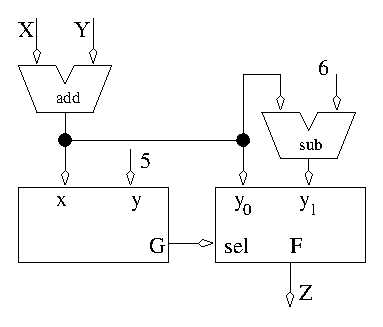
\includegraphics{Sol4-11}

                    }
                \end{onlysolution}

            \item \textbf{ (1pt. each)}Convert the following to 2's-complement
                assuming a word size of eight bits.
                \begin{enumerate}
                    \item -35

                        \begin{onlysolution} \textbf{Solutions} \itshape{
                                $35 = 32+2+1 = 100011 = 00100011$, thus $-35=11011101$
                            }
                        \end{onlysolution}

                    \item  -128

                        \begin{onlysolution} \textbf{Solutions} \itshape{
                                This is a special case, see page 10 for more information.
                                $-128 = 10000000$
                            }
                        \end{onlysolution}

                    \item  67

                        \begin{onlysolution} \textbf{Solutions} \itshape{
                                $67=64+2+1 = 100 0011 = 0100 0011$
                            }
                        \end{onlysolution}

                    \item  128

                        \begin{onlysolution} \textbf{Solutions} \itshape{
                                There are not enough bits to represent this positive number; hence
                                the 8-bit representation does not exist.
                            }
                        \end{onlysolution}

                \end{enumerate}

            \item \textbf{ (1 pt. each)} Perform the following operations for the given
                2's-complement numbers. Assume a word size of eight bits
                in all cases. Indicate where overflow occurs. If there is no overflow,
                convert the result to decimal.
                \begin{enumerate}

                    \item 01011101 + 00110111

                        \begin{onlysolution} \textbf{Solutions} \itshape{
                                01011101 + 00110111 = 10010100  overflow
                            }
                        \end{onlysolution}

                    \item 11101011 + 11110001

                        \begin{onlysolution} \textbf{Solutions} \itshape{
                                11101011 +
                                11110001 =
                                11011100
                            }
                        \end{onlysolution}

                    \item 01011101 + 10101011

                        \begin{onlysolution} \textbf{Solutions} \itshape{
                                01011101 +
                                10101011 =
                                00001000
                            }
                        \end{onlysolution}

                    \item 10111011 - 11110001

                        \begin{onlysolution} \textbf{Solutions} \itshape{
                                10111011 -
                                11110001 =

                                10111011 +
                                00001111 =
                                11001010
                            }
                        \end{onlysolution}

                    \item 01011101 - 00110111

                        \begin{onlysolution} \textbf{Solutions} \itshape{
                                01011101 -
                                00110111 =

                                01011101 +
                                11001001 =
                                00100110
                            }
                        \end{onlysolution}

                    \item 01011101 - 10101111

                        \begin{onlysolution} \textbf{Solutions} \itshape{
                                01011101 -
                                10101111 =

                                01011101 +
                                01010001 =
                                10101110, overflow
                            }
                        \end{onlysolution}

                \end{enumerate}

            \item \textbf{ (10 pts.)}
                \label{page:flipbox}
                Build a flip box.  A flip box is defined by the following input,
                output, and behavior definition.

                \begin{tabular}{|l|p{3.5in}|} \hline
                    Nomenclature:  & 8-bit flip box.                    \\ \hline
                    Data Input:    & 8-bit $D=d_7 \ldots d_0$          \\ \hline
                    Data Output:   & 8-bit $F=f_7 \ldots f_0$          \\ \hline
                    Control:       & 3-bit $S=s_2 s_1 s_0$            \\ \hline
                    Status:        & none                                   \\ \hline
                    Behavior:      & The output is the same as the input except for
                    one bit which is inverted.  The index of the inverted
                    bit is given by $S$. \\ \hline
                \end{tabular}

                The flip box takes the 8-bit data input, flips a single bit identified
                by $S$, then sends the new 8-bit value to the output.
                For example, if $D=11110000$ and $S=010$ then
                $F=11110100$.  If $D=11110000$ and $S=101$ then $F=11010000$.  The solution
                should rely heavily on the basic building blocks.

                \begin{onlysolution} \textbf{Solutions} \itshape {
                        Arrange 8, 2:1 muxes with $d_i$ and $d_i'$ going into the data inputs.
                        Run the select into a 3:8 decoder and route the data outputs to the
                        individual selects of the 2:1 muxes.
                    }
                \end{onlysolution}

            \item \textbf{ (10 pts.)}
                \label{page:IsScan}
                Build a box which recognizes some keyboard scancode.  When a key is
                pressed on a keyboard, the keyboard transmits (among other things)
                an 8-bit scancode of the pressed key.  Each key has its own scancode
                listed in Table~\ref{table:scancodes}.  The relationship between the
                keys and their scancode is not based on ASCII.

                \begin{table}
                    \begin{tabular}{|l|l||l|l||l|l||l|l|} \hline
                        Key & scancode & Key & scancode & Key & scancode & Key & scancode \\ \hline \hline
                        0 & $45_{16}$ & 1 & $16_{16}$ & 2 & $1E_{16}$ & 3 & $26_{16}$ \\ \hline
                        4 & $25_{16}$ & 5 & $2E_{16}$ & 6 & $36_{16}$ & 7 & $3D_{16}$ \\ \hline
                        8 & $3E_{16}$ & 9 & $46_{16}$ & A & $1C_{16}$ & B & $32_{16}$ \\ \hline
                        C & $21_{16}$ & D & $23_{16}$ & E & $24_{16}$ & F & $2B_{16}$ \\ \hline
                        P & $4D_{16}$ & L & $4B_{16}$ & M & $3A_{16}$ & I & $43_{16}$ \\ \hline
                    \end{tabular}
                    \caption{Some keyboard scancodes.}
                    \label{table:scancodes}
                \end{table}

                \label{page:scanclass}
                \begin{tabular}{|l|p{3.5in}|} \hline
                    Nomenclature:  & scancode classifier                   \\ \hline
                    Data Input:    & 8-bit $D=d_7 \ldots d_0$          \\ \hline
                    Data Output:   & IsP, IsL, IsM, IsI, IsS \\ \hline
                    Control:       & none             \\ \hline
                    Status:        & none                                   \\ \hline
                    Behavior:      & IsP =1 when $D$ is the scan code for the letter ``P".
                    IsL =1 when $D$ is the scan code for the letter ``L".
                    IsM =1 when $D$ is the scan code for the letter ``M".
                    IsI =1 when $D$ is the scan code for the letter ``I".
                    IsS =1 when $D$ is the scan code for the letter ``S".  \\ \hline
                \end{tabular}

            \item \textbf{ (10 pts.)}
                \label{page:ScanDecode}
                Build a box which converts an 8-bit scancode for a hexadecimal
                digit into a 4-bit hexadecimal values.

                \label{page:scanconv}
                \begin{tabular}{|l|p{3.5in}|} \hline
                    Nomenclature:  & scancode classifier                   \\ \hline
                    Data Input:    & 8-bit $D=d_7 \ldots d_0$          \\ \hline
                    Data Output:   & 4-bit $H=h_3h_2h_1h_0$ \\ \hline
                    Control:       & none             \\ \hline
                    Status:        & none                                   \\ \hline
                    Behavior:      & Converts the scancode $D$, representing a the
                    key of a hexadecimal character, into its 4-bit
                    value $H$.
                    \\ \hline
                \end{tabular}

                For example, if $D=25_{16}$, the scancode for the "4" key, then the converter
                should output $H=0100_2$.  Assume that the inputs are always
                legal hexadecimal scancodes.

        \end{enumerate}
